\documentclass[conference, onecolumn]{IEEEtran}     % Comments after  % are ignored
\usepackage{amsmath,amssymb,amsfonts} % Typical maths resource packages
\usepackage{graphics}                 % Packages to allow inclusion of graphics
\usepackage{color}                    % For creating coloured text and background
\usepackage{hyperref}                 % For creating hyperlinks in cross references

\oddsidemargin 0cm
\evensidemargin 0cm

\pagestyle{myheadings}         % Option to put headers
                               % Needed \documentclass[a4paper,twoside]{article}



%\markboth{{\small\it PDF\ \LaTeX \ coloured text and graphics}}

%{{\small\it C.T.J. Dodson} }
\textwidth 15.5cm
\topmargin -1cm
\parindent 0cm
\textheight 24cm
\parskip 1mm

\newtheorem{theorem}{Theorem}[section]
\newtheorem{proposition}[theorem]{Proposition}
\newtheorem{corollary}[theorem]{Corollary}
\newtheorem{lemma}[theorem]{Lemma}
\newtheorem{remark}[theorem]{Remark}
\newtheorem{definition}[theorem]{Definition}



\def\R{\mathbb{ R}}

\def\S{\mathbb{ S}}




\date{\small\it April 20, 2009}

\title{{Power / Delay Estimation of \\ Auto Generated Circuits}}

%\footnote{A demonstration example including colored text and graphics}}}





\author{ K. P. Ghosh, S.Subramanian \\
{\small Department of Electrical Engineering, IIT, Bombay, India}
 }










\begin{document}

\pagenumbering{arabic}
\maketitle
\begin{abstract}

The goal of the research project was to characterize RTL generated by the AHIR flow.
We have taken a set of examples, used AHIR to generate RTL, mapped the RTL to layout and finally performed power, area and delay estimation for the above examples.
For all our circuit examples we have used the OSU Standard Cell library for TSMC 0.18 technology and Synopsis  Design Compiler to perform synthesis.
The netlist thus obtained is used as an input to Cadence SOC Encounter to generate the layout.
The layout being closest to the actual hardware is most suiatble for estimation of power consumed in the design for a particular input sequence.
Five examples viz. A5, AES, Red Black trees, Linpack and FFT were selected, six memory architectures were explored for each and results are summarized in final section.


\end{abstract}

\section{Introduction}
AHIR provides a platform to translate an algorithm described in a high level programming language like C to a VHDL circuit description. In this work, we characterise the resulting hardware in terms of physical and performance parameters such as area, power and delay. Our approach followed for obtaining layout from a VHDL description is as shown in the Fig. 1.


\begin{figure}[ht]
{\centering \resizebox*{6in}{4in}{\includegraphics{list_of_figures1.ps}} \par}
\caption{Flow describing VHDL Description to Layout}
\end{figure}

At each level, a different tool is used for a specific purpose. At first,  the VHDL code is simulated and checked for  its functionality using ModelSim 6.3a. The next step is  to perform synthesis and obtain a gate level netlist. For all our circuit examples we have used the OSU Standard Cell library for TSMC 0.18 technology and Synopsis  Design Compiler (DC) to perform synthesis. The netlist thus obtained is used as an input to Cadence SOC Encounter to generate the layout. 

The memory is designed as single bank or as a combination of multiple banks. The later would aid parallelism in the circuit. Also, the memory could be pipelined. We have explored 6 different memory architectures for different examples and compared the performance of the circuits with multiple banks versus single banks, pipelined as opposed to non-pipelined memory. 

\section{Memory Modelling}
Memories has been treated as blackboxes due to the absence of SRAM cells in the OSU standard cell library.
For SOC Encounter to estimate power, delay and area of the entire hardware, the memory black boxes must have the required information. We use Cacti 3.2[1] to estimate power and delay in the memory blackboxes. The area is modelled using the following expression[2].

area(in mm2) = (0.001){ * }(tech)^{2.07} { * } (bits)^{0.9} { * } (port)^{0.7} + {0.0048}

The values of power, area and delay obtained from the above models are used to generate the necessary information for the blackboxes in timing library file (TLF) and library exchange file (LEF) formats. The vital timing information is also obtained from delay models. 

To describe a memory element as a black box, we instruct Synopsys DC to turn off its synthesis when it encounters the architecture for the memory.
Thus for Synopsys DC, the memory is an entity definition with well defined input and output ports but a blank architecture.
Similarly, Cadence SOC Encounter is made to infer black boxes whenever a memory component is instantiated from the TLF and LEF files.

\section{Power Estimation}
The layout being closest to the actual hardware is most suitable for estimation of power consumed in the design for a particular input sequence.
Power has been calculated using SOC Encounter.

Using the final gate level verilog netlist provided by SOC Encounter we perform a post -layout simulation and dump all the signal information to a vcd file. This vcd file is used by SOC Encounter to generate a power report. One is also required to mention the top level entity name for which power is to be estimated.

Circuits like Linpack, Redblack have larger memory requirement and also take long time to simulate. For such examples, a sampling technique was followed, in order to reduce the size of VCD files (which was around 25Gb). In this technique, the final post layout netlist is simulated and the switching activities are captured at 10 random intervals of time. It was observed that, when power is calculated using these samples, the variance in power estimates for the samples is negligible.  

\section{Results}
Five examples viz. A5, AES, Red Black trees, Linpack and FFT were selected. 
The memory architecture choices are shown TABLE I:

\begin{table}[t]

\caption{Architecture choices for each example}
\begin{center}
{\begin{tabular}{c  c | c  c  c}
\hline
ARCHITECTURE && \multicolumn{3}{c}{MEMORY BANK CHOICE} \\  
CHOICES && 1& 2& 4 \\ [3ex] 
\hline
Example& Memory Size &&Base Bank Address Width \\ [1ex]
\hline 
A5& 16& 4& 4& 4\\[1ex]
LINPACK& 16K& 12& 12& 12\\[1ex]
R-B TREES& 16k& 12& 12& 12\\[1ex]
FFT& 512& 8& 8& 8\\[1ex]
AES& 1024& 8& 8& 8\\[1ex]
\hline

\end{tabular}}
\label{diffstruc}
\end{center}	
\end{table}

For each of memory architecture choices, deeply pipelined and non-pipelined was selected.
The range of frequencies tried for each architecture is shown in TABLE II:


\begin{table}[t]
\caption{Range of Frequencies for Each Architecture}
\begin{center}
{\begin{tabular}{c | c  c  c  c  c  c}
\hline
 & \multicolumn{6}{c}{ARCHITECTURE CHOICES} \\[1ex]
 &1x2 &1x0 &2x0 &2x2 &4x2 &4x0 \\ [1ex]
\hline
Example& \multicolumn{6}{c}{Frequency of Operation (in MHz)} \\ [1ex]
\hline
A5& 71.42& 71.42& 83.33& 71.42& 83.33& 71.43\\[1ex]
LINPACK& 45.45& 41.67& 41.67& 41.67& 41.67& 38.4\\[1ex]
R-B TREES& 41.67 and 62.5 & 41.67 and 55.56& 71.42& 50& 71.42& 38.36\\[1ex]
FFT& 41.66& 41.66& 41.66& 45.45& 45.45& 45.45\\[1ex]
AES& 45.45 and 71.42& 45.45 and 71.42& 71.42& 71.42& 71.42& 45.45\\[1ex]
\hline

\end{tabular}}
\\[1ex]
Note : Architecture choices are in the form [memory bank x deeply pipelined/non-pipelined degree]. For eg. 4 x 2 indicates an architecture with number of memory banks as 4. 2 and 0 indicates pipelined and non-pipelined memory, repectively.
\label{diffstruc}
\end{center}
\end{table}

\subsection{Reports}
The energy, delay and area estimates for each example are as follows:

\subsubsection{A5/1}
\\
The energy, delay and area estimates for each architecture / frequency combination is given in TABLE III.
In Fig. 2,  Fig. 3 we show the Power-Delay and Area-Delay plot for A5/1. 
\begin{table}[h!]
\caption{Energy / Delay / Area for each architecture/frequency combination}
\begin{center}
{\begin{tabular}{c | c   c   c   c    c   c}
\hline
A5/1 &1x2 &1x0 &2x0 &2x2 &4x2 &4x0 \\ [1ex]
\hline
Frequency (MHz) & 71.42& 71.42& 83.33& 71.42& 83.33& 71.42 \\ [1ex]
Energy (nJ) &25.26 &20.44 &29.484 &22.078 &34.56 &23.436 \\ [1ex]

Delay (ns)& 308& 280& 252& 266& 240& 252\\[1ex] 
Area (mm^2)& 1.45& 1.3& 1.77& 1.52& 2.3& 1.9\\[1ex]
\hline

\end{tabular}}
\label{diffstruc}
\end{center}
\end{table}


\begin{figure}[h!]
{\centering \resizebox*{6in}{4in}{\includegraphics{a5p.ps}} \par}
\caption{Power-Delay plot for A5/1}
\end{figure}

\begin{figure}[h!]
{\centering \resizebox*{6in}{4in}{\includegraphics{a5a.ps}} \par}
\caption{Area-Delay plot for A5/1}
\end{figure}


\subsubsection{LINPACK}
\\
The energy, delay and area estimates for each architecture / frequency combination is given in TABLE IV.
In Fig. 4, Fig. 5 we show the Power-Delay and Area-Delay plot for Linpack.

\begin{table}[h!]
\caption{Energy / Delay / Area for each architecture/frequency combination}
\begin{center}
{\begin{tabular}{c | c   c   c   c    c   c}
\hline
LINPACK &1x2 &1x0 &2x0 &2x2 &4x2 &4x0 \\ [1ex]
\hline
Frequency (MHz) & 45.45& 41.67& 41.67& 41.67&41.67 & 38.4\\[1ex]
Energy (mJ) &18.92 &11.47 &22.75 &10.28 &29.53 &11.07 \\ [1ex]

Delay (ms)& 56.48& 43.65& 55.63& 37.68& 51.64& 38.71\\[1ex] 
Area (mm^2)& 27.5& 25.5& 30.8& 27& 36.2& 28.9\\[1ex]
\hline

\end{tabular}}
\label{diffstruc}
\end{center}
\end{table}


\begin{figure}[h!]
{\centering \resizebox*{6in}{4in}{\includegraphics{lpp.ps}} \par}
\caption{Power-Delay plot for LINPACK}
\end{figure}

\begin{figure}[h!]
{\centering \resizebox*{6in}{4in}{\includegraphics{lpa.ps}} \par}
\caption{Area-Delay plot for LINPACK}
\end{figure}




\subsubsection{R-B TREES}
\\
The energy, delay and area estimates for each architecture / frequency combination is given in TABLE V.
In Fig. 6, Fig. 7 shows the Power-Delay and Area-Delay plot for Red-Black Trees.

\begin{table}[h!]
\caption{Energy / Delay / Area for each architecture/frequency combination}
\begin{center}
{\begin{tabular}{ c |c  c  c  c   c   c    c   c}
\hline
R-B TREES &\multicolumn{2}{c}{1x2} &\multicolumn{2}{c}{1x0} &2x0 &2x2 &4x2 &4x0 \\ [1ex]
\hline
Frequency (MHz)& 41.67& 62.5& 41.67& 55.56& 71.42& 50 & 71.42&38.36\\[1ex]
Energy (mJ)&3.935 & 7.062 &1.511 &2.54 &8.07 &2.851 &11.47  &3.23 \\ [1ex]

Delay (ms)& 18.74 & 12.5& 9.88 & 7.41& 10.9& 8.17& 10.87& 10.57\\[1ex] 
Area (mm^2)& 19 & 23& 18 & 21& 26& 22& 32& 25\\[1ex]
\hline

\end{tabular}}
\label{diffstruc}
\end{center}
\end{table}


\begin{figure}[h!]
{\centering \resizebox*{6in}{4in}{\includegraphics{rbp.ps}} \par}
\caption{Power-Delay plot for RED-BLACK TREES}
\end{figure}

\begin{figure}[h!]
{\centering \resizebox*{6in}{4in}{\includegraphics{rba.ps}} \par}
\caption{Area-Delay plot for RED-BLACK TREES}
\end{figure}





\subsubsection{FFT}
\\
The energy, delay and area estimates for each architecture / frequency combination is given in TABLE VI.
In Fig. 8, Fig. 9 we show the Power-Delay and Area-Delay plot for FFT.

\begin{table}[ht]
\caption{Energy / Delay / Area for each architecture/frequency combination}
\begin{center}
\begin{tabular}{c | c   c   c   c    c   c}
\hline
FFT &1x2 &1x0 &2x0 &2x2 &4x2 &4x0 \\ [1ex]
\hline
Frequency (MHz) &41.66 &41.67& 41.66& 45.45& 45.45&45.45 \\ [1ex] 
Energy (uJ)&24.65 &14.71 &31.04 &16.7 &41.38 &18.55 \\ [1ex]

Delay (us)& 203.792& 154.88& 189.27& 141.606& 172.453& 140.55\\[1ex] 
Area (mm^2)& 5.4& 5.07 & 6.6& 5.7& 9.2& 6.7\\[1ex]
\hline

\end{tabular}}
\label{diffstruc}
\end{center}
\end{table}


\begin{figure}[ht]
{\centering \resizebox*{6in}{4in}{\includegraphics{fftp.ps}} \par}
\caption{Power-Delay plot for FFT}
\end{figure}

\begin{figure}[ht]
{\centering \resizebox*{6in}{4in}{\includegraphics{ffta.ps}} \par}
\caption{Area-Delay plot for FFT}
\end{figure}





\subsubsection{AES}
\\
The energy, delay and area estimates for each architecture / frequency combination is given in TABLE VII.
In Fig. 10, Fig. 11 we show the Power-Delay and Area-Delay plot for AES.

\begin{table}[h!]
\caption{Energy / Delay / Area for each architecture/frequency combination}
\begin{center}
{\begin{tabular}{c | c c c c c c c c}
\hline
AES &\multicolumn{2}{c}{1x2} &\multicolumn{2}{c}{1x0} &2x0 &2x2 &4x2 &4x0 \\ [1ex]
\hline
Frequency (MHz)& 45.45&71.42 & 45.45& 71.42& 71.42& 71.42& 71.42& 45.45 \\ [1ex]
Energy (uJ) &310.97 & 386.03 &147.38 & 144.664 &560.07 &157.58 &846.28 &177.5 \\ [1ex]

Delay (ms)& 1.21& 0.769& 0.67 & 0.43& 0.762& 0.418& 0.759& 0.655\\[1ex] 
Area (mm^2)& 7.67 & 9.03& 6.63 & 6.5 & 13& 7.5& 20.25& 9.4\\[1ex]
\hline
\end{tabular}}
\label{diffstruc}
\end{center}
\end{table}


\begin{figure}[h!]
{\centering \resizebox*{6in}{4in}{\includegraphics{aesp.ps}} \par}
\caption{Power-Delay plot for AES}
\end{figure}

\begin{figure}[h!]
{\centering \resizebox*{6in}{4in}{\includegraphics{aesa.ps}} \par}
\caption{Area-Delay plot for AES}
\end{figure}




\clearpage

\section{Conclusion}

From the results, tabulated and plotted earlier, we can conclude the following:
\begin{enumerate}
\item The nonpipelined memory looks more efficient in power-delay and area-delay, when compared to the deeply pipelined case. 
There's no significant improvement in delays as we increase the number of banks except A5/1.
This indicates that there is limited parallelism in the memory accesses.
\item The circuits are usually more energy efficient at higher frequency of operation.
\item The floating point operators limit the higher operating frequency in the case of FFT and Linpack.
\item Energy per operation for FFT and Linpack is in the order of 10 nJ and 12 nJ respectively. 
\end{enumerate}



\addcontentsline{toc}{chapter}{References}
\begin{thebibliography}{99}

\bibitem{} Premkishore Shivakumar, Norman P. Jouppi. Cacti 3.0 : An Integreted Cache Timing, Power, and Area model,
{\bf Western Research Laboratory}, 250 University Avenue Palo Alto, California 94301 USA.


\bibitem{} Banit Agrawal, Timothy Sherwood. Guiding Architectural SRAM models, 
{\bf Published in International Conference of Computer Design (ICCD) 2006},Department of Computer Science, University of California, Santa Barbara.


\end{thebibliography}



\end{document}

